%% Adapted from `tikzposter-example.tex',

%% Modify the size of the paper for the usual 4 ft x3 ft poster size
\PassOptionsToPackage{paperwidth=48in, paperheight=36in,
  textwidth=48in, textheight=36in,
  innermargin=1in, margin=.25in,
  centering}{geometry}
\PassOptionsToPackage{dvipsnames}{xcolor}
\documentclass[25pt, landscape,blockverticalspace=0.5in, colspace=0.5in, subcolspace=0.33in]{tikzposter} %Default values for poster format options.
\tikzposterlatexaffectionproofoff % remove tikzposter logo

%% fonts: helvetica + palatino
% Euler for math | Palatino for rm | Helvetica for ss | Courier for tt
\renewcommand{\rmdefault}{ppl} % rm
\linespread{1.05}        % Palatino needs more leading
\usepackage[scaled]{helvet} % ss
\usepackage{courier} % tt
%\usepackage{euler} % math
\usepackage{eulervm} % a better implementation of the euler package (not in gwTeX)
\normalfont
\usepackage[T1]{fontenc}
\renewcommand{\familydefault}{\sfdefault} % use sans-serif

%%%% OTHER IMPORTANT PACKAGES
\usepackage{amsmath, amsthm, amssymb} %AMS math
\usepackage{bm}% bold math
\usepackage{color} % colored text
\usepackage[pdftex,colorlinks=true,
allcolors=blue
]{hyperref}% add hypertext capabilities
\usepackage{paralist}% for compactitem used by Marko
\usepackage{multirow}% multicolumn/row cells in tables
\usepackage{url} % add auto-linked urls
\usepackage{mathtools} % shortintertext, and other useful math-related features
\usepackage{siunitx} % SI units
\sisetup{per-mode = symbol}
\usepackage[dvipsnames]{xcolor}
\usepackage{pgfplots}
\pgfplotsset{compat=newest}

% choose one bibliography package:
\usepackage[backend=bibtex,citestyle=numeric-comp]{biblatex}
%\usepackage{amsrefs} % references
%%%%

\addbibresource{bibliography.bib} % bibliography file

% Title, Author, Institute
\usetitlestyle{Envelope}
\title{A most excellent research project}
\author{First Author$^1$, Second Author$^2$}
\institute{${}^1$ Clarkson, ${}^2$ Not Clarkson}


% -- PREDEFINED THEMES ---------------------- %
 % Choose LAYOUT:  Default, Basic, Rays, Simple, Envelope, Wave, Board, Autumn, Desert,
 \usetheme{Autumn}

 % colors based on Clarkson visual identity guide
 % rotating colorOne/Two/Three and the countries below leads to various color themes
 \definecolorpalette{Clarkson}{ 
   \definecolor{colorOne}{HTML}{004E42}
   \definecolor{colorTwo}{HTML}{D7D2CB}   
   \definecolor{colorThree}{HTML}{FFCD00}
 }
 
% options: Default, Australia, Britain, Sweden, Spain, Russia, Denmark, Germany 
\usecolorstyle[colorPalette=Clarkson]{Germany} % try Spain for easy alternative

\usetitlestyle{Filled}
 \begin{document}

 \maketitle
 \node[anchor=west] at (TP@title.west) {\hspace{3in}\includegraphics[height=3in]{logos/clarkson-seal.png}};
 \node[anchor=east] at (TP@title.east) {\includegraphics[height=2in]{logos/clarkson-logo.png} \hspace*{2in}};


 \begin{columns}%blocks will be placed into columns

       \column{.33}

       \block{Title}{


         Math:
         \[
           \int_0^t f(x(\tau))d\tau 
         \]

         We can also put a graph in and refer to it here: Fig.~\ref{fig:first}
         \begin{tikzfigure}[This is a graph.]\label{fig:first}
           \includegraphics[width=0.5\linewidth]{figs/graph}
         \end{tikzfigure} 

       }


       \column{.33}

       \block{Methods}{
         Something common.

         \coloredbox{Important statement can be highlighted}
       }

     
       \begin{subcolumns}
         \subcolumn{.5}
         \block{Type 1}{
           Something cited from
           \cite{Hill1894}
         }
         \subcolumn{.5}
         \block{Type 2}{
           Something else}

       \end{subcolumns}

       \block{More}{
         For more information, take a look at \texttt{tikzposter-example.tex} and \texttt{tikzposter-example.pdf} in this folder. 
       }
       \note[targetoffsetx=2in, angle=-45,targetoffsety=0in,connection]{Additionally, documentation for the poster class is in \url{https://ctan.org/pkg/tikzposter}.}


       \column{.33}

       \block{Results}{
Most people get matrices wrong (overly complicated) in \LaTeX. This is the right way:
\[ %this produces unenumerated equation.
  \begin{bmatrix}
    1 & 2y \\
    \ast & 3x
  \end{bmatrix}
\]


\begin{tikzfigure}[Title]
   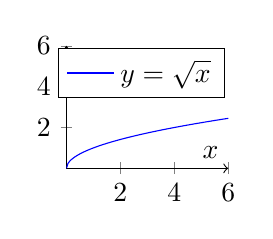
\begin{tikzpicture}
     \begin{axis}[
       xmin=0, xmax=6,
       xlabel={$x$},
       ymin=0, ymax=6,
       ylabel={$y$},
       axis lines=middle,
       axis line style=->,
       width=.3\linewidth]
        \addplot[no marks,blue,-,domain=0:6, samples=100] expression{sqrt(x)};
        \addlegendentry{$y=\sqrt{x}$};
      \end{axis}
   \end{tikzpicture}
 \end{tikzfigure}
}

       
       \block{References}{
         \printbibliography[heading=none]
       }

     \end{columns}



 \end{document}




\endinput
%%
%% End of file `tikzposter-example.tex'.
